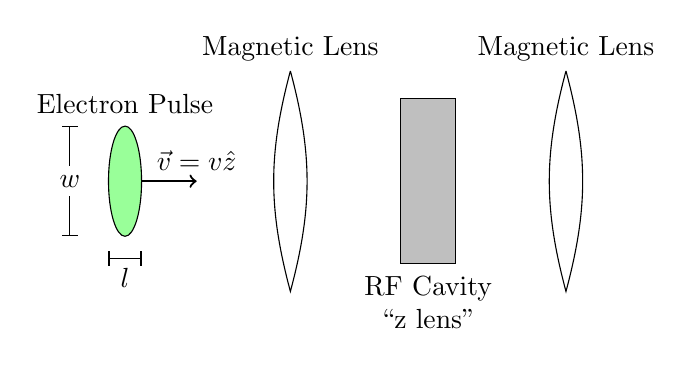
\begin{tikzpicture}[scale=0.7]
  \draw [fill=green!40] (0,0) ellipse [x radius=3mm, y radius=1cm];
  \draw [|-|] (-1,1) -- ++(0,-2) node [pos=0.5,fill=white] {$w$};
  \draw [|-|] (-0.3,-1.4) -- ++(0.6,0) node [pos=0.5,below] {$l$};
  \node at (0, 1.4) {Electron Pulse};
  \draw [thick, ->] (0.3,0) -- ++ (1,0) node [above,pos=1] {$\vec{v} = v \hat{z}$};
  \draw 
    (3,2)
    to [out=-75,in=75] ++(0,-4)
    to [out=105,in=255] ++(0,4)
    node [above] {Magnetic Lens}
  ;
  \draw [fill=gray!50] (5,1.5) rectangle ++(1,-3);
  \node at (5.5,-2.2) [align=center] {RF Cavity\\``z lens''};
  \draw 
    (8,2)
    to [out=-75,in=75] ++(0,-4)
    to [out=105,in=255] ++(0,4)
    node [above] {Magnetic Lens}
  ;
\end{tikzpicture}
